\pgfplotstablegetelem{\thepart}{[index]\columnIndex}\of{\cronograma}
\part{\pgfplotsretval}
\label{part:\thepart}
\frame{\partpage}



\begin{frame}[t]{Programação Orientada a Objetos (POO)}
	
	\fontsize{14pt}{15}\selectfont{
		
		Os principais elementos da \acrshort{poo} são os objetos. Dizemos que um objeto é uma instância de uma classe. Uma \textbf{Classe} é constituída por variáveis (membros de dados) e métodos ou funções (membros da função).
		
	}\par
	\vspace{2em}
	
	\fontsize{14pt}{25}\selectfont{
		\begin{itemize}%[<+->]  
			\item A Classe é o modelo. Um objeto é um elemento deste modelo.
			
			\item As variáveis de uma Classe são também chamadas de \textbf{Atributos}.
			
			\item As funções de uma Classe são também chamadas de \textbf{Métodos}.
			
		\end{itemize}
	}\par
	\vspace{1em}
	
	
\end{frame}



\begin{frame}[t]{Objetivos da POO}
	
	\vspace{1em}
	
	\fontsize{14pt}{25}\selectfont{
		\begin{itemize}%[<+->]  
			\item Robustez – o programa não pode cair frente a dados inesperados.
			\item Adaptabilidade – rodar facilmente em diferentes ambientes.
			\item Reusabilidade – usar os elementos já construídos em outros sistemas.
			
		\end{itemize}
	}\par
	\vspace{1em}
	
	\fontsize{10pt}{15}\selectfont{
	\href{https://wiki.python.org.br/GuiaDeEstilo}{Python Enhancement Proposals (PEP, em português, Propostas de Melhoria do Python) 8 - Guia de Estilo Para Python - pt-br}\\
	\href{https://peps.python.org/pep-0008/}{PEP 8 – Style Guide for Python Code - inglês}
	
	*obs: PEP é um conjunto de convenções e práticas para a linguagem de código Python, essas práticas tem uso difundido na comunidade Python e facilitam a compreensão e edição do seu código.
	}\par

\end{frame}


\begin{frame}[t]{Objetivos da POO}
	
	\fontsize{14pt}{15}\selectfont{
		
		
	}\par
	\vspace{2em}
	
	\fontsize{14pt}{25}\selectfont{
		\begin{itemize}%[<+->]  
			\item Eles representam entidades em sua aplicação em desenvolvimento.
			
			\item As entidades interagem entre si para resolver problemas do mundo real.
			
			\item Por exemplo, Produto é uma entidade, Carro tamém é uma entidade. 
			
		\end{itemize}
	}\par
	\vspace{1em}
	
	
\end{frame}



\begin{frame}[t]{Classes}
	
	\fontsize{14pt}{15}\selectfont{
		
		As classes ajudam os desenvolvedores a representar entidades do mundo real:
		
	}\par
	\vspace{1em}
	
	\fontsize{14pt}{15}\selectfont{
		\begin{itemize}%[<+->]  
			\item As classes definem objetos com atributos e comportamentos. Os atributos são membros de dados e os comportamentos são manifestados pelas funções-membro.
			
			\item As classes são constituídas de construtores que proporcionam o estado inicial para esses objetos.
			
			\item As classes são como templates, portanto, podem ser facilmente reutilizadas.
			
		\end{itemize}
	}\par
	\vspace{1em}
	
	
	*obs: Por exemplo, a classe Produto tem atributos nome e quantidade e uma função-membro que altera a quantidade do produto.
	
\end{frame}




\begin{frame}[t]{Vamos praticar}
	

	\vspace{1em}
	
	\centering
%	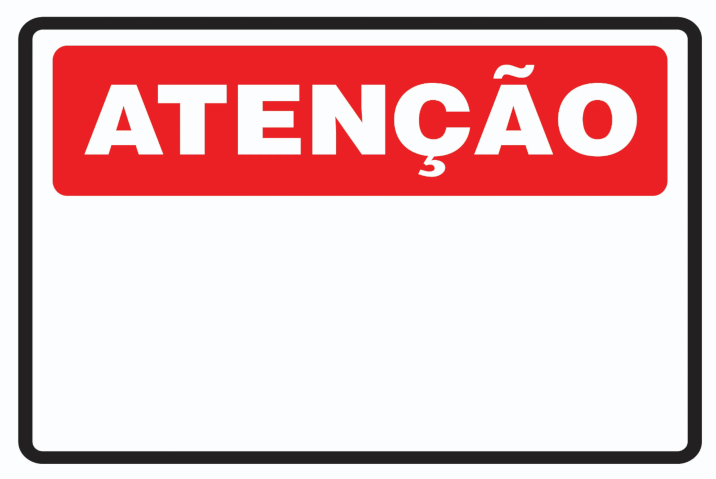
\includegraphics[scale=0.25]{imagens/fig-atencao-fundo-branco.png}
	
	\begin{tikzpicture}
		\node (image) {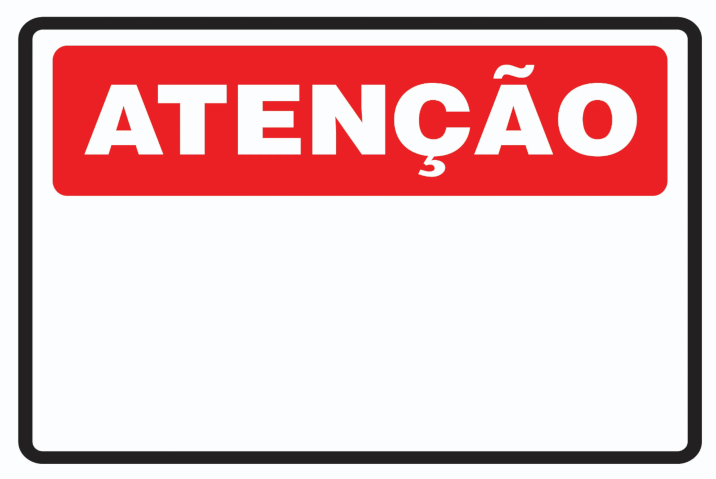
\includegraphics[width=7cm]{imagens/fig-atencao-fundo-branco.png}};
		\node [x={(image.south east)},y={(image.north west)}] at (0,0){Vamos escrever um algoritmo};
	\end{tikzpicture}

	
\end{frame}


\begin{frame}[t]{Vamos praticar - Algoritmo}
		
	\vspace{1em}
	
	\fontsize{14pt}{19}\selectfont{
		\begin{itemize}%[<+->]  
			\item Início
			\item Abrir um bloco de notas (qualquer recurso para escrever).
			\item Escolha um objeto (pode ser algo do seu dia a dia).
			\item Escreva duas das principais características desse objeto.
			\item Escreva duas das principais ações desse objeto.
			\item Escreva em um bloco de notas.
			\item Salve em arquivo que vamos utilizar até o final da aula de hoje.
			\item Fim
			
		\end{itemize}
	}\par
	\vspace{1em}
	
\end{frame}



\begin{frame}[t]{Vamos praticar - Algoritmo}
	
	
	\fontsize{14pt}{15}\selectfont{
		Solução...		
	}\par
	\vspace{1em}
	
	\fontsize{14pt}{19}\selectfont{
		\begin{itemize}%[<+->]  
			\item Objeto escolhido: Carro
			\item Duas características: 
				\begin{itemize}%[<+->]
					\item Cor
					\item Modelo
				\end{itemize}
			\item Duas ações:
				\begin{itemize}%[<+->]
					\item Acelerar
					\item Frear
				\end{itemize}
			
		\end{itemize}
	}\par
	\vspace{1em}
	
\end{frame}


\begin{frame}[t]{Vamos praticar - Algoritmo}
	
	
	\fontsize{14pt}{15}\selectfont{
		Solução...		
	}\par
	\vspace{1em}
	
	\fontsize{14pt}{19}\selectfont{
		\begin{itemize}%[<+->]  
			\item Objeto escolhido: Produto \textbf{(classe)}
			\item Duas características: \textbf{(atributos)}
			\begin{itemize}%[<+->]
				\item Preço
				\item Quantidade
			\end{itemize}
			\item Duas ações: \textbf{(métodos)}
			\begin{itemize}%[<+->]
				\item Alterar Preço
				\item Alterar Quantidade				
			\end{itemize}
			
		\end{itemize}
	}\par
	\vspace{1em}
	
\end{frame}


\begin{frame}[t]{Princípios da POO}
	
	\fontsize{14pt}{15}\selectfont{
		
		
	}\par
	\vspace{1em}
	
	\fontsize{14pt}{25}\selectfont{
		\begin{itemize}%[<+->]  
			\item Modularidade – dividir o sistema em pequenas partes bem definidas.
			
			\item Abstração – identificar as partes fundamentais (tipos de dados e operações), definindo o que cada operação faz e não necessariamente como é feito.
			
			\item Encapsulamento – a interface para uso de cada componente deve estar bastante clara para todos que usam esse componente. Detalhes internos de implementação não interessam.
			
		\end{itemize}
	}\par
	\vspace{1em}
	
	
\end{frame}




\begin{frame}[t]{O desenvolvimento de software}
	
	%	\fontsize{14pt}{15}\selectfont{
		%		
		%		Não há uma regra, método ou processo que oriente o desenvolvimento de bons programas e sistemas de	computador. 
		%		
		%	}\par
	\vspace{1em}
	
	\fontsize{12pt}{15}\selectfont{
		\begin{itemize}%[<+->]  
			\item Há apenas diretrizes gerais que quando usadas levam em geral a um bom resultado. 
			
			\item O desenvolvimento certamente é influenciado pelo ambiente computacional no qual será desenvolvido. 
			
			\item A	linguagem de programação e o ambiente ou plataforma na qual será desenvolvido o sistema podem decidir o	modo, a estratégia e os passos que serão usados.
			
		\end{itemize}
	}\par
	\vspace{1em}
	
	
\end{frame}



\begin{frame}[t]{O desenvolvimento de software}
	
	\fontsize{14pt}{15}\selectfont{
		
		Podemos dividir o desenvolvimento de software em 3 etapas, independente da linguagem, sistema operacional ou plataforma de desenvolvimento que será usada.
		
	}\par
	\vspace{1em}
	
	\fontsize{12pt}{15}\selectfont{
		\begin{itemize}%[<+->]  
			\item O projeto.
			
			\item A implementação.
			
			\item Os testes e depuração.
			
		\end{itemize}
	}\par
	\vspace{1em}
	
	
\end{frame}




\begin{frame}[t]{O desenvolvimento de software}
	
	\fontsize{14pt}{15}\selectfont{
		
		O projeto é a parte mais importante. Nele são definidas as classes e a relação entre elas. Os princípios que devem orientar a definição das classes são:
		
	}\par
	\vspace{1em}
	
	\fontsize{12pt}{15}\selectfont{
		\begin{itemize}%[<+->]  
			\item \textbf{Responsabilidade de cada uma delas} – quais problemas elas resolve.
			
			\item \textbf{Independência entre elas} – se uma precisa da outra e vice-versa.
			
			\item \textbf{Comportamento} – quais as entradas (parâmetros) e saídas (resultados) das classes.
			
		\end{itemize}
	}\par
	\vspace{1em}
	
	
	
\end{frame}





\begin{frame}[t]{Resumo sobre Programação Orientada a Objetos}
	
	\fontsize{10pt}{15}\selectfont{
		
		Os princípios básicos da \acrshort{poo} são descritos a seguir.
		
	}\par
	\vspace{0.5em}
	
	\fontsize{10pt}{12}\selectfont{
		\begin{itemize}%[<+->]  
			\item \textbf{Classe}: Representação de um conjunto de objetos com características afins. Definição do comportamento dos objetos (métodos) e seus atributos. 
			
			\item \textbf{Objeto}: Uma instância de uma classe. Armazena estados por meio de atributos e reação a mensagens enviadas por outros objetos.
			
			\item \textbf{Abstração}: Oculta detalhes que não são necessários no contexto.
			
			\item \textbf{Herança}: Mecanismo pela qual uma classe (sub-classe) pode estender outra classe (super-classe), estendendo seus comportamentos e atributos.
			
			\item \textbf{Polimorfismo}: Princípio pelo qual as instâncias de duas classes ou mais classes derivadas de uma mesma super-classe podem invocar métodos com a mesma assinatura, mas com comportamentos distintos. 
			
			\item \textbf{Encapsulamento}: Proibição do acesso direto ao estado de um objeto, disponibilizando apenas métodos que alterem esses estados na interface pública. 
			
			\item \textbf{Composição}: É uma maneira de combinar objetos ou classes. Na composição, um objeto é usado para chamar função-membro sem o uso de herança.
			
		\end{itemize}
	}\par
	\vspace{1em}
	
\end{frame}




\begin{frame}[t]{Um exemplo de programação orientada a objeto com Python}
	
	\fontsize{13pt}{15}\selectfont{
		
		Vamos desenvolver um sistema que possui produtos. O objeto em questão é o produto. Assim, vamos criar a classe Produto, que tornará possível construir ou criar elementos ou objetos desta classe.
		
	}\par
	\vspace{0.5em}
	
	A sintaxe básica para criação de uma classe é´:
	
	\vspace{0.5em}
	\begin{beamercolorbox}[wd=\textwidth]{warning}
		class {NomeDaClasse}: \\
		\hspace{1em}{Instruções}
	\end{beamercolorbox}
	
	\vspace{0.5em}
	\fontsize{11pt}{15}\selectfont{
		\begin{itemize}%[<+->]  
			\item \textbf{classe} - Produto.
			
			\item \textbf{atributos} - nome, codigo, preco, quantidade.
			
			\item \textbf{métodos} - obtem\_nome, obtem\_codigo, obtem\_preco, altera\_preco, altera\_quantidade.
			
		\end{itemize}
	}\par
	\vspace{0.5em}
	
	\url{https://docs.python.org/pt-br/3/tutorial/classes.html}
	
\end{frame}


\begin{frame}[t]{Requisitos da classe Produto}
	
	\fontsize{14pt}{15}\selectfont{
		
		Vamos listar abaixo:
		
	}\par
	\vspace{1em}
	
	
	\fontsize{12pt}{15}\selectfont{
		\begin{itemize}%[<+->]  
			\item Deve ser possível recuperar o nome, código e preço do produto.
			
			\item Devolve True se novo preço for maior que o atual preço.
			
			\item Devolve False se a quantidade de produtos requerida não está disponível.
			
		\end{itemize}
	}\par
	\vspace{1em}
	
	
\end{frame}



\begin{frame}[t]{Atenção}
	
	%	\vspace{1em}
	%	\fontsize{14pt}{19}\selectfont{
		%		Escreva utilizando algoritmo.
		%	}\par
	%	
	%	\vspace{1em}
	%	
	%	\centering
	%	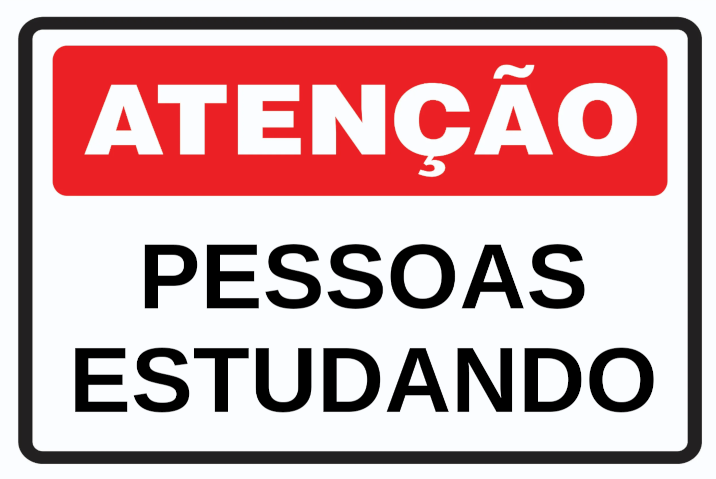
\includegraphics[scale=0.4]{imagens/fig-atencao-pessoas-estudando.png}
	
	%	\parbox{1\linewidth}{ 
		\centering
		\begin{tikzpicture}
			%		\node at (0,0){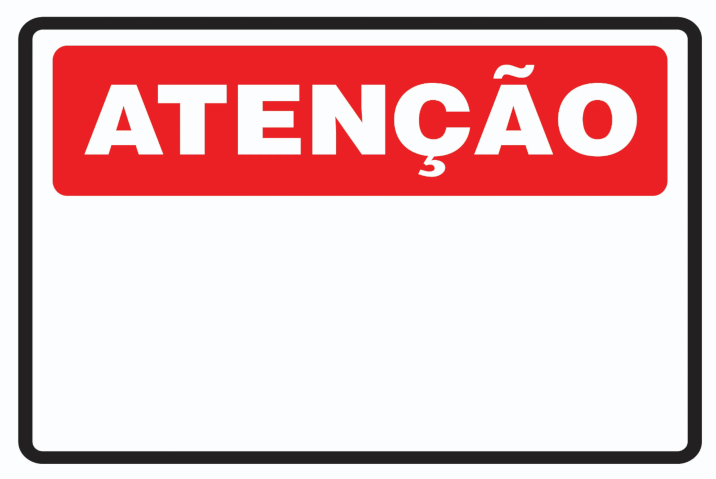
\includegraphics[width=0.7\textwidth]{imagens/fig-atencao-fundo-branco.png}
				\node (image) 
				{
					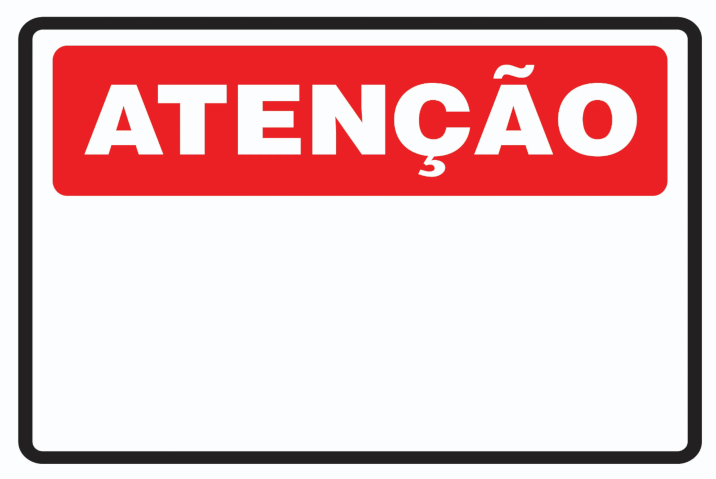
\includegraphics[width=0.7\textwidth]{imagens/fig-atencao-fundo-branco.png}
				};
				\node
				[
				%		fill=teal,
				overlay,
				align=center,
				text=black,
				font={\fontsize{34pt}{19}\bfseries}
				] at (0,-1) (image.center) {Respirem fundo\\ que vamos...};
			\end{tikzpicture}
			%	}
		
		
	\end{frame}
	
	
	
	\begin{frame}[t]{Exemplos de criação de classe}	
		
		\lstinputlisting[style=CBruno,caption=Código da classe Produto]{outros/codigos/python/codigo_003_classe_produto.py}
		
		\vspace{1em}
		
		
	\end{frame}
	
	
	\begin{frame}[t]{Exemplos de criação de classe}	
		
		
		\fontsize{14pt}{15}\selectfont{
			
			Se o código abaixo for colocado junto com o arquivo da classe Produto, é posssível "testar" o código no mesmo arquivo. É desaconselhável fazer.
			
		}\par
		\vspace{1em}
		
		\fontsize{14pt}{25}\selectfont{
			\begin{beamercolorbox}[wd=\textwidth]{warning}
				if \_\_name\_\_ == "\_\_main\_\_":\\
				\hspace{1em}p1 = Produto("Laranja", 1, 1.56, 10)\\
				\hspace{1em}print("Oferta do dia:", p1.obtem\_nome())\\
				\hspace{1em}if p1.altera\_preco(40.00): print("Preco alterado hoje")\\
				\hspace{1em}else: print("Atencao - baixou o preco")
			\end{beamercolorbox}
			
		}\par
		\vspace{1em}
		
	\end{frame}
	
	
	
	
	\begin{frame}[t]{Pytest}
		
		\vspace{-2em}
		\lstinputlisting[style=CBruno,caption=Cobertura de testes da classe Produto]{outros/codigos/python/test_codigo_003_classe_produto.py}
		
		
		
	\end{frame}
	
	
	
	\begin{frame}[t]{Pytest}
		
		
		\vspace{1em}
		\centering
		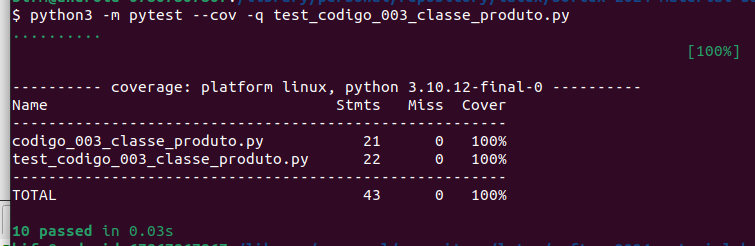
\includegraphics[scale=0.5]{imagens/fig-result-test-class-produto.png}
		
	\end{frame}
	
	
	
	
	\begin{frame}[t]{classe Produto}
		
		\fontsize{14pt}{15}\selectfont{
			
			O nome \textbf{self} refere-se ao particular objeto sendo criado. Note que o primeiro parâmetro é sempre self na definição. No uso ou na chamada do método esse primeiro parâmetro não existe.
			
		}\par
		\vspace{1em}
		
		
		\fontsize{12pt}{15}\selectfont{
			\begin{itemize}%[<+->] 
				
				\item No exemplo anterior incluímos além da definição da classe, alguns comandos de teste dos métodos da mesma. Assim o módulo (arquivo onde está armazenada a classe) poderia chamar-se Produto.py.
				
				\item O comando if \textbf{\_\_name\_\_} == “\textbf{\_\_main\_\_}” usado antes dos testes anteriormente, determina que os comandos abaixo somente serão executados quando a classe estiver sendo testada, isto é, quando for solicitada a execução do módulo Produto.py
				
			\end{itemize}
		}\par
		\vspace{1em}
		
		
	\end{frame}
	
	
	
	
